
\section{Results}

The model was tested in several scenarios. First, the price 
dynamics and order book evolution are studied with a simple one market settings in which the dividend
yield and interest rate are set to zero. Then the same aspects are investigated
using more complex settings: only some of the traders are allowed to place orders
per trading session and the dividend yield and interest rate are set to random walk.
Then arbitrage is studied using 
a setting in which there exists two identical markets.


\subsection{Single asset simulation}
% Price dynamics, stylized facts, order book evolution
The single asset simulation was run twice: first run
was conducted with a starting market price of 500 and second
with a starting market price of 1500. The simulations were
run with 500 traders trading 1000 rounds. The 
amount of currency and the amount of stock 
a trader owns in the beginning of the simulation were set to
10 000 000 and 10 000 respectively. Therefore
the ratio of stock to currency is 1 000 which
is the expected equilibrium price as there are
no payouts in either asset. The amount of currency
per trader may seem much but as the tick size is one,
it may be more convenient to think the currency in amounts
in cents or pennies. The standard deviation of
the price each trader bids and asks with is set to 20. The 
starting market price was set to 400 to study the 

% Descriptive analysis
The evolution of trade prices, quantities and values thorough
the trading sessions for both simulations are shown in the figure
~\ref{fig:basic_trades}. As can be observed,
the near equilibrium market price is achieved in around 20 trading
sessions for both runs. The reason why the price stays slightly 
under the equilibrium price may be caused by the implementation of
determining the order price and order quantity. If a trader decides
to allocate less currency on an order than the decided order price 
the order gets obviously invalidated but there is no such
limitation for placing asks. Therefore there might be a slightly less
bids than asks in general. 

\begin{figure}
    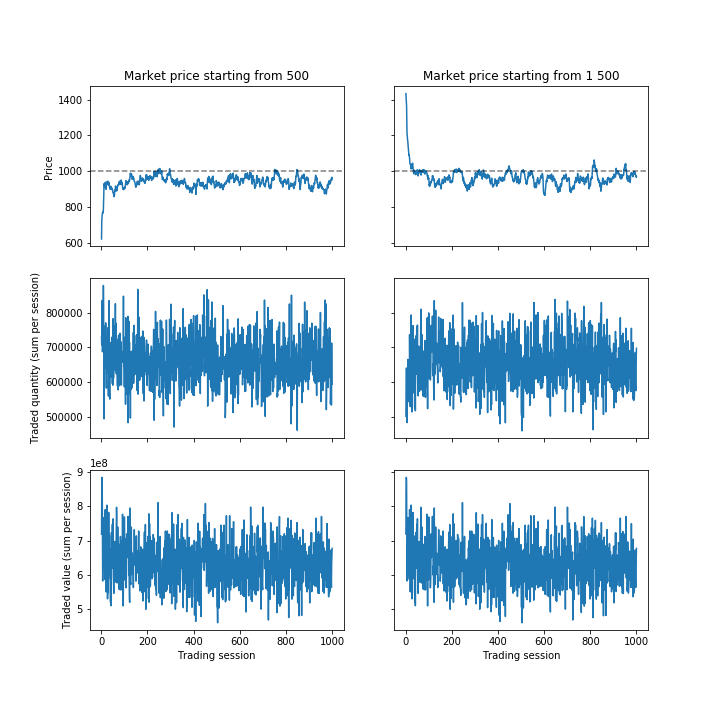
\includegraphics[width=\linewidth]{plots/basic_trades.png}
    \caption{Evolution of price and quantity}
    \label{fig:basic_trades}
\end{figure}

% How the market converged to equilibrium
The market depths shown in figure ~\ref{fig:market_depths} suggests that the
converge to equilibrium is caused by balancing the sides of the market. 
In the figure the order book is visualized for the first 100 trading sessions. 
The surface describes the evolution of the cumulative bids and cumulative asks 
thorough time and the bottom of the valley in the surface is the bid-ask spread. 
The left side from the valley is the the bid book and the right is the ask book. The 
ask side of the market is almost completely missing initially in the run that
starts with lower market price while the opposite is true for the run with higher
initial market price. The side emerges rapidly after few trading session
and the market price approaches near equilibrium price and vice versa for the 
simulation starting with higher market price. An example of the market depth 
when the equilibrium is reached is shown in ~\ref{fig:basic_market_depth_equilibrium}.


\begin{figure}
    \centering
    \begin{subfigure}{.5\textwidth}
      \centering
      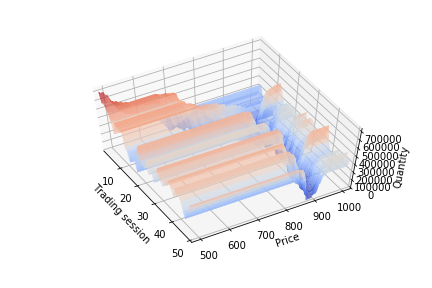
\includegraphics[width=\linewidth]{plots/basic_market_depth_converge_lower.png}
      \caption{Starting price 500}
      \label{fig:market_depth_lower}
    \end{subfigure}%
    \begin{subfigure}{.5\textwidth}
      \centering
      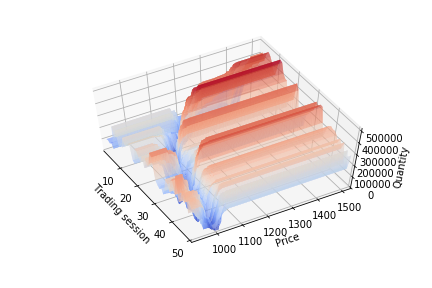
\includegraphics[width=\linewidth]{plots/basic_market_depth_converge_higher.png}
      \caption{Starting price 1 500}
      \label{fig:market_depth_higher}
    \end{subfigure}
    \caption{Converge of the order book to equilibrium}
    \label{fig:market_depths}
\end{figure}

\begin{figure}
    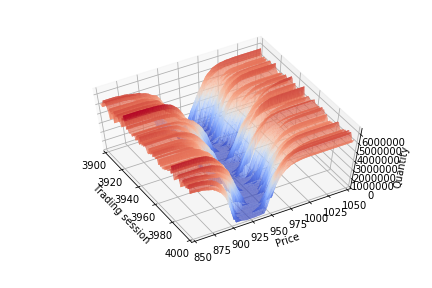
\includegraphics[width=\linewidth]{plots/basic_market_depth_in_equilibrium.png}
    \caption{Market depth when equilibrium reached (last 50 sessions)}
    \label{fig:basic_market_depth_equilibrium}
\end{figure}

% stylized facts
% Somethging about filtering fist 100 out and now inspecting stylized facts
As stated before, the representativeness of real markets is inspected using
stylized facts. In order to have represenative data set to test the facts, the
sessions before reaching the price equilibrium are filtered out. 
As observed in ~\ref{fig:basic_trades}, the model reaches the equlibrium 
price before the 100th trading session and after that both of the initiations 
yield similar price and quantity processes. Therefore, for simplicity the
the first 100 trading sessions are filtered out from the simulation with
lower initiated market price and the data produced from it is used for 
studying the stylized facts in the model.

The autocorrelation function (ACF) and partial autocorrelation function (PACF) for the last prices of
each session are plotted in the figure ~\ref{fig:basic_autocorr}. ACF and PACF indicate that there is 
an autoregressive (AR) process for up to 15 lags and a moving average (MA) process to the third lag. Therefore
there is a clear autocorrelation in the model with the stated simulation parameters. This
observation is possibly caused by option for doing nothing which occurs with slightly higher than
one-third probability due to slight chance for invalid order submission. As the price in each order
is dependent on the market price which existed when the order was created and as there is a chance that
this order will stay in the order book for some time, the market price in the past has influence on the
current structure of the order book and therefore a past market prices have effect on the upcoming prices.
This phenomenon can be interpret from the figure ~\ref{fig:basic_market_depth_equilibrium}: the valley
formed by the sides of the order book resembles river. In case of no autocorrelation, one would expect
that there would be no clear continuous valley formed by the order book and the spread would change
its location more intensively. 
% NOT TRUE, autocorrelation found when there is no option for "inaction"
% Maybe the reason is that when the price gets lower, less has 

This indicates that if the zero intelligent traders are given the option to not change their orders and
the market is structured as continuous double auction, autocorrelation may be inevitable. Either the
rationality of the traders regarding to when they decide to do nothing should be increased, the option
to do nothing should be taken off or limit the lifetime of an order in order to reduce the autocorrelation.
In addition, \citet{StylizedFacts01} also discussed that in the real markets there may be autocorrelation 
of returns for small intraday time periods, such as 20 minutes, due to market microstructure and therefore
one trading session in the simulation may be more closer, in terms of interpretation, to a smaller period 
than one day.
% Something about intra day autocorrelation in real markets. Maybe if a trading session is considered as
% trading hour, the simulation is more realistic?

\begin{figure}
    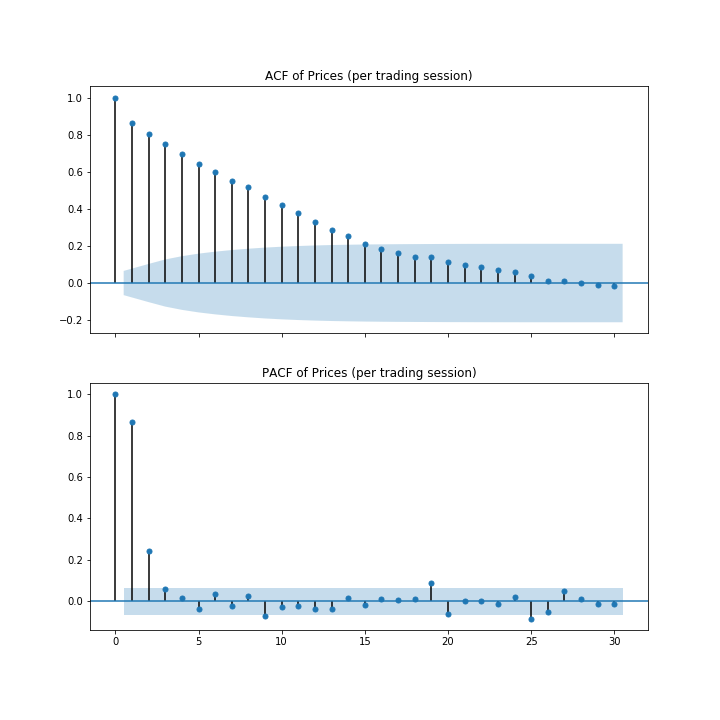
\includegraphics[width=\linewidth]{plots/basic_autocorrelation.png}
    \caption{Autocorrelation of the simulation after 100 session}
    \label{fig:basic_autocorr}
\end{figure}

% Fat-tailed returns
The returns are, however, fat-tailed as can be observed from figure 
~\ref{fig:basic_return_fitdistr}. The distribution of returns decay
initially rapidly when moving from the mean compared to the fitted
normal distribution but the tails of the distributions stretch
further due to high kurtosis. However, the distribution does have
significantly higher spike in the mean than what is observed, for 
example, in the figure~\ref{fig:sp_fat_tails} regarding to S\&P500's
fat tails. 
% basic_fat_tails_cumdist


\begin{figure}
    \centering
    \begin{subfigure}{.5\textwidth}
      \centering
      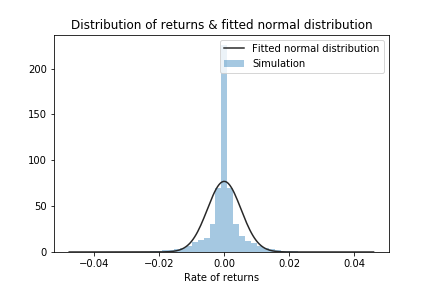
\includegraphics[width=\linewidth]{plots/basic_fat_tails.png}
      \caption{Return distribution}
      \label{fig:basic_return_fitdistr}
    \end{subfigure}%
    \begin{subfigure}{.5\textwidth}
      \centering
      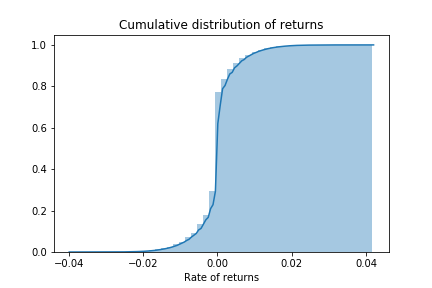
\includegraphics[width=\linewidth]{plots/basic_fat_tails_cumdist.png}
      \caption{Return cumulative distribution}
      \label{fig:basic_return_cumdistr}
    \end{subfigure}
    \caption{Return distributions after 100 sessions}
    \label{fig:basic_return_distr}
\end{figure}


% Volatility clusters
The autocorrelation of the volatilities in figure ~\ref{fig:basic_volaclusters}
indicate there are some volatility clusters in short term. Both, ACF and PACF, shows slow
decay indicating that there are both of the autocorrelation terms, AR and MA,
present in the volatility of the market price. The effect is, however, rather short term
as it is not carried over trading sessions as shown in the appendix ~\ref{app:basic_volaclusters_per_session}


\begin{figure}
    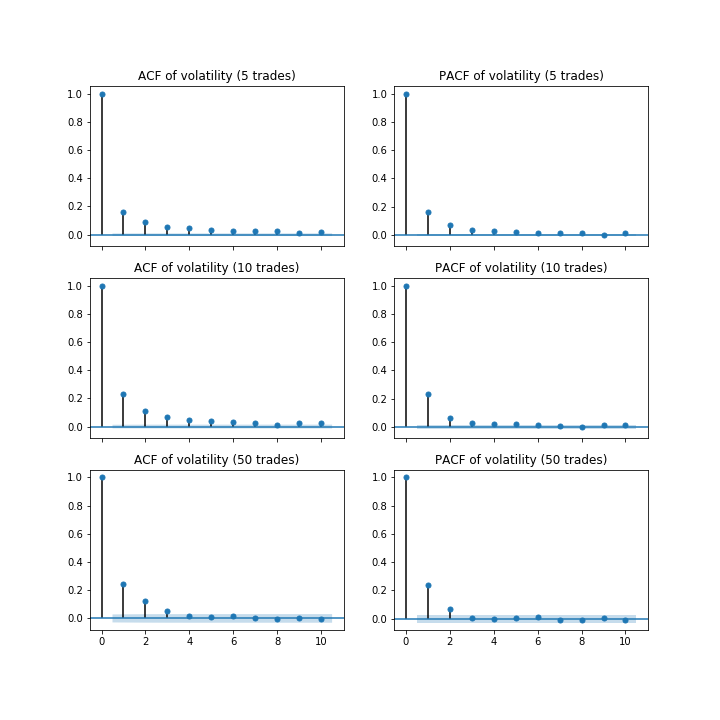
\includegraphics[width=\linewidth]{plots/basic_volaclusters_intraday.png}
    \caption{Volatility Clusters}
    \label{fig:basic_volaclusters}
\end{figure}

\subsection{Arbitrage simulation}

To 
